\section{Chokepoint Measures}


\begin{figure}
	\centering
	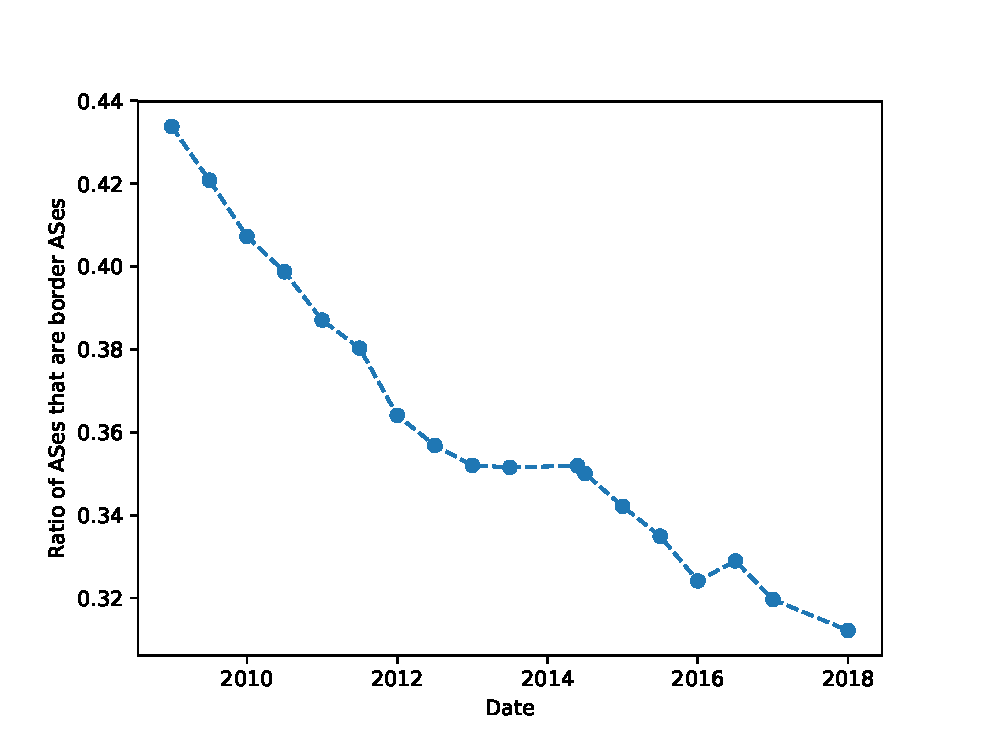
\includegraphics[width=\linewidth]{bnodes}
	\caption{The ratio of ASes that are border ASes plotted over several years.}\label{fig:bnodes}
\end{figure}

\begin{figure}
	\centering
	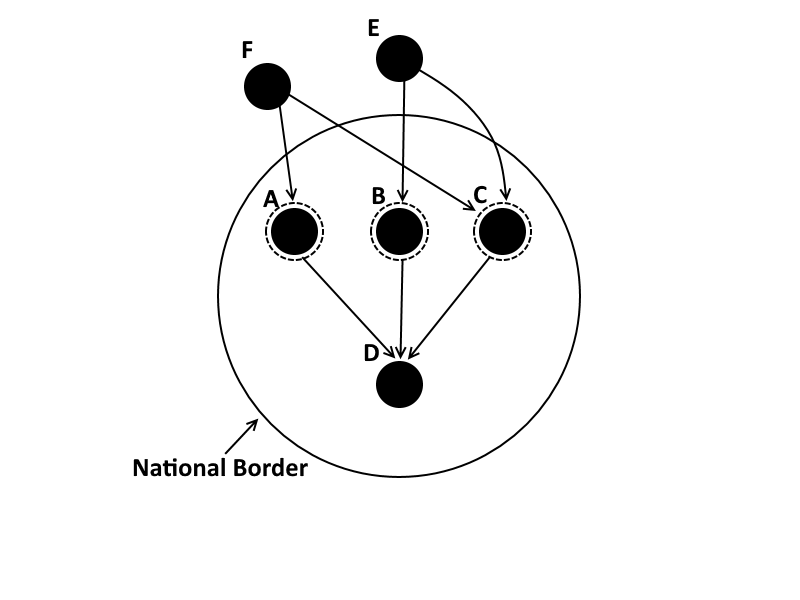
\includegraphics[width=\linewidth]{chokepoint}
	\caption{Chokepoint potential example. ASes A,B, and C are all border ASes. 
						AS D is an internal AS. ASes E and F are both external ASes.
						The out-to-in chokepoint potentials of A,B, and C are 0.25, 0.25, and 0.5 respectively.}\label{fig:chokepoint}
\end{figure}


Border ASes are ASes that lie one hop from an AS registered to a different country. It stands to reason that if information bottlenecks
were to be implemented by national governments, they would likely be implemented on border ASes. This is not always true, but there are more reasons
to use border ASes as our unit of investigation. For instance, the ratio of the number of border ASes of
a country to all ASes in that country hints toward the abillity of that nation to intercept information flows across their borders.
\figurename \ref{fig:bnodes} shows that globally the number of border ASes has grown at a slower rate to the number of non-border ASes
over time so that the ratio of border ASes to ASes has almost continuously decreased. On the surface it would seem that this fact reflects an ever increasing capability for nations to intercept AS-level paths. This is not
neccessarily the case, however. Because AS-level paths are generated by the distributed BGP and the local preferences of AS administrators often do not
lead to simple shortest path selections, a better way to understand the potential for bottlenecks on border ASes is to investigate the number of BGP generated
paths that pass through each AS. To do this we propose an intuitive measure on border ASes called \emph{chokepoint potential}. Since this is a measure for single ASes
we also need an aggregate measure for comparing nations, which we call \emph{national breakthrough potential}.

% % Why Border ASes?
% In order to identify AS chokepoints and compare nations, we need a measure that can be calculated from the many paths between
% ASes. First, we decided to use a measure that is evaluated only on border ASes, or ASes that lie one hop from an AS belonging to another nation. 
% The evolution of AS relationships and national boundaries on the AS graph hints that border ASes are an important feature in regards to the flow
% of information. Consider that while the number of ASes globally has continued to grow rapidly, the number of border ASes has grown more slowly.
% This result is depicted in figure \ref{fig:bnodes}. Additionally, while internal chokepoints may intercept many paths, those paths are required
% to have entered through a border AS (in the case of out-to-in paths) or exit through a border AS (for in-to-out paths). This focus on border ASes has
% the added benefit of making calculations more efficient.

\par
For our measures we use the term \textit{path} to indicate a path that is generated by BGP consisting of a source AS, a destination AS, and the intermediate
ASes between them. We define a \textit{routing tree} to be a tree rooted at a single destination AS and composed of every acceptable BGP path from the various source ASes that can reach the destination AS.
We define the chokepoint potential of a border AS to be the ratio of paths intercepted by that border AS
to the number of paths intercepted by all border ASes belonging to the same nation. For instance, take a border AS $b$, belonging to country $c$.
If $P_c$ is the set of paths in to or out of country $c$ and $B_p$ is the set of border ASes within path $p$, then the
chokepoint potential of $b$, $CP(b)$ is defined formally in equation \ref{eqn:chokePointPotential}. This measure captures
the relative strength exhibited by a border AS in regards to what portion of paths it intercepts. This is calculated
seperately for in-to-out paths (those starting from a source in the country in question) and out-to-in paths. The out-to-in chokepoint potential for a simple dummy nations
is included in \figurename \ref{fig:chokepoint}.

% Formal Definition
\begin{equation}\label{eqn:chokePointPotential}
CP(b) = \frac{|\{p \in P_c \textrm{ s.t. } \{b\} \subseteq B_p\}|}{\sum_{p \in P_c}|B_p|}
\end{equation}

\par
Given a set of routing trees, chokepoint potential is an intuitive way to compare individual ASes. With this measure,
the sum of the chokepoint potential for all border ASes for a country is 1.0, as in, all of the border ASes collectively control the
flow of information over the nation's border. To compare one nation to another, we can inspect how many border ASe minimum are required
to obtain a certain chokepoint potential. The more border ASes required, the more difficult it would likely be for that nation to perform
censorship or surveillance, as the government would have to restrict more ISPs, place more filtering hardware, etc. Thus, we can define
another measure, with this one being a national measure. We define the \emph{national breakthrough potential} of a nation to be the minimum number
of ASes required to intercept a selected percentage of AS-level paths. Previous work has used 90\% path interception as a benchmark indicating strong control
of information \cite{throats}, so we use this percentage as well. When used here, however, 90\% path interception indicates a single nation intercepts 90\% of the paths
that either enter said nation (for the out-to-in case) or exit said nation (for the in-to-out case). National breakthrough potential is calculated taking the strongest ASes first,
such that the measure reflects the smallest number of border ASes needed to intercept the paths. We use the number of ASes here and not a percentage because using a percentage would
make it difficult to compare nations. Take for instance the United States, which has many more ASes than most nations. If the United States and another nation both required the same percentage
of border ASes to intercept 90\% of paths, the similarity of these nations would be misleading, because the United States would actually need to control many more ASes.
Our technique provides a comparison more likely to reflect reality. This measure is called a breakthrough potential because it indicates the number of border ASes that intercept a vast majority of paths, meaning that a country with high NBP would require controlling many border ASes to prevent a breakthrough, or an unfettered access of
internal ASes to that country.
